 \section{Questões}
\begin{enumerate}
 \item (Sociesc - 2009) Um grupo de escoteiros foi acampar. Do acampamento avistaram o pico de um morro segundo um ângulo de $30 \degree$. Ao caminharem mais 30 metros em direção ao morro passaram a ver o pico segundo um ângulo de $60 \degree$. Sendo $\sen 30\degree = \frac{1}{2}$, $\cos 30\degree =\frac{\sqrt{3}}{2}$, $\sen 60\degree =\frac{\sqrt{3}}{2}$, $\cos 60\degree =\frac{1}{2}$, $tg 60\degree = \sqrt{3}$ e $tg 30\degree =\frac{\sqrt{3}}{3}$ , altura do morro é:
 \begin{multicols}{2}

 \begin{enumerate}
  \item 15 metros
  \item $\frac{30}{\sqrt{3}-1}$ metros
  \item $\frac{30\sqrt{3}}{1-\sqrt{3}}$ metros
  \item $15\sqrt{3}$ metros
 \end{enumerate}

 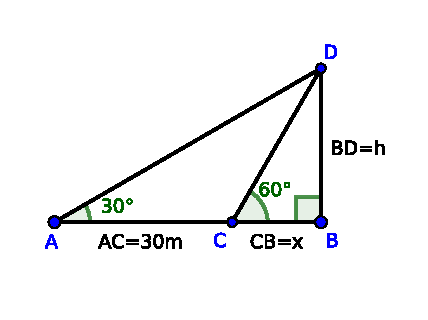
\includegraphics[width=6cm]{../../Topicos/Figuras/tri_ret_exer.pdf}

 \end{multicols}

 \item (Sociesc - 2010) Uma rampa lisa de 24 m de comprimento faz ângulo de $60\degree$ com o plano horizontal. Uma pessoa que sobe essa rampa inteira atinge o ponto mais alto verticalmente de:

  Dados: $\sen (60\degree)= \frac{\sqrt{3}}{2}$, $\cos (60\degree)= \frac{1}{2}$, $\tan (60\degree)= \sqrt{3}$
 \begin{multicols}{2}

 \begin{enumerate}
  \item $\frac{17 \sqrt{3}}{2} m$
  \item $15\sqrt{3} m$
  \item $12\sqrt{3} m$
  \item $\frac{25 \sqrt{3}}{2} m$
  \item $18\sqrt{3} m$
 \end{enumerate}

 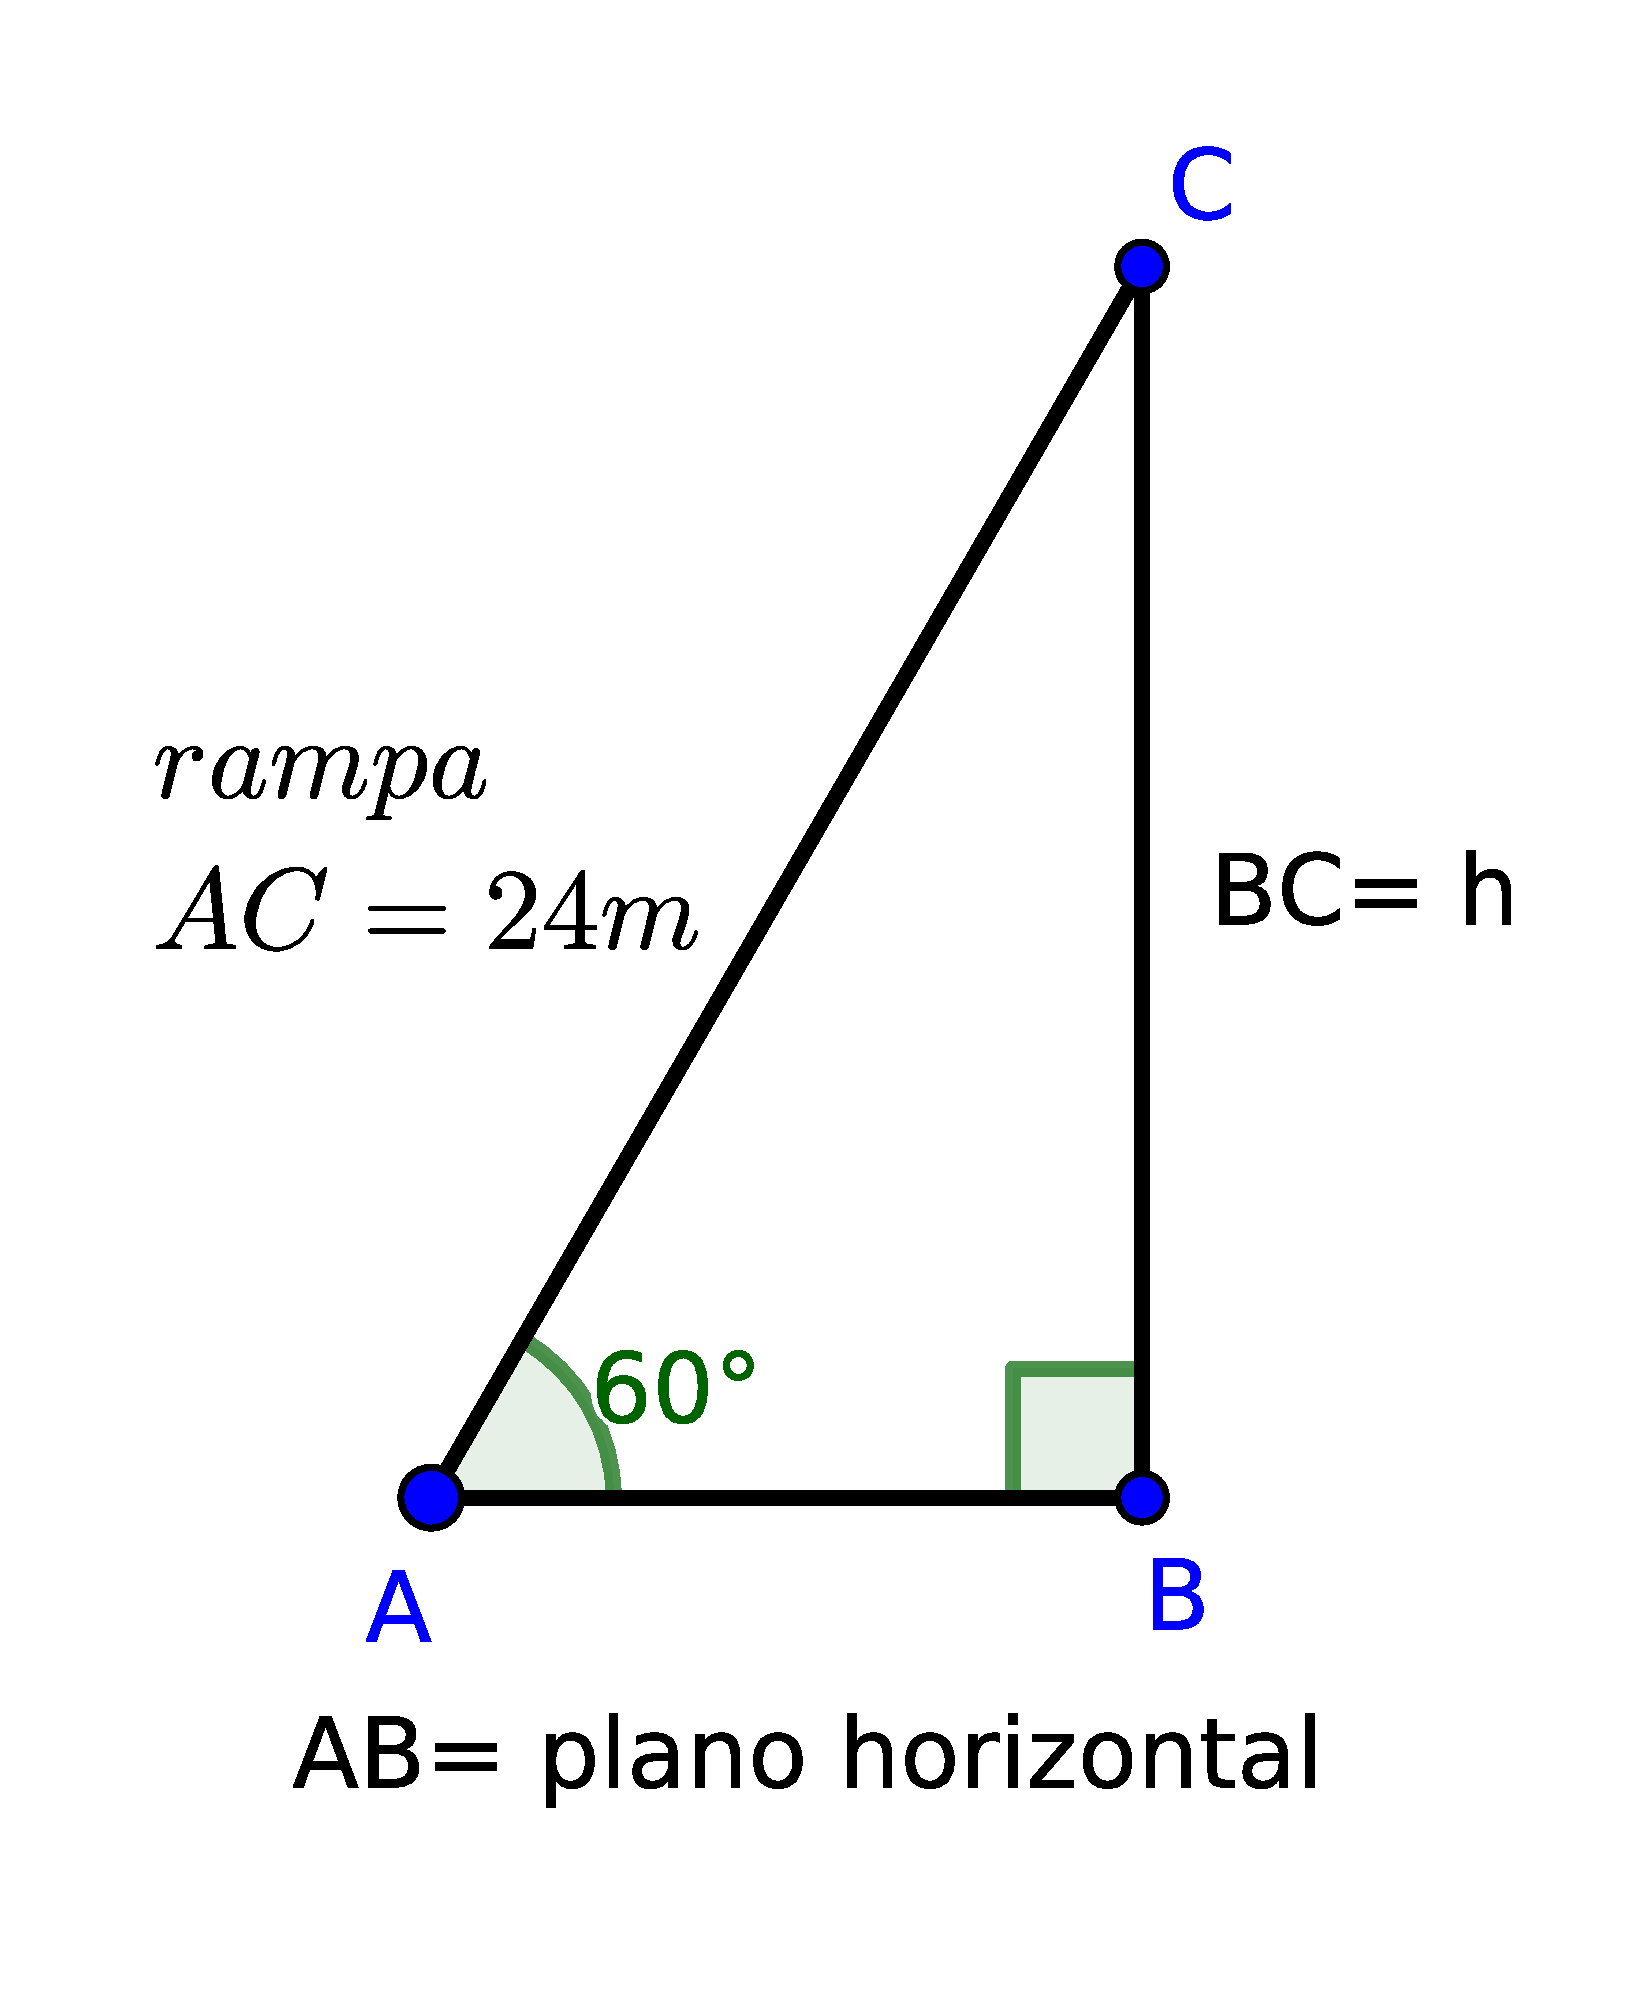
\includegraphics[width=4cm]{../../Topicos/Figuras/tri_ret_exer2.pdf}
 \end{multicols}

 \item (Sociesc - 2010) Um teleférico deve unir os topos A e B de dois morros. Para calcular a quantidade de cabo necessário foi preciso medir a altura dos morros em relação a um plano horizontal, obtendo-se 108m e 144m respectivamente. A seguir, mediu-se o ângulo que a reta $\overline{AB}$ forma com a horizontal, obtendo-se $32\degree$. Calcule a distância entre os pontos A e B, sabendo que $\sen (32\degree)= 0,52$, $\cos (32\degree)= 0,84$ e $\tan (32\degree)= 0,62$.

 \begin{multicols}{2}

 \begin{enumerate}
  \item 18,72 m
  \item 48,23 m
  \item 69,23 m
  \item 78,45 m
 \end{enumerate}

 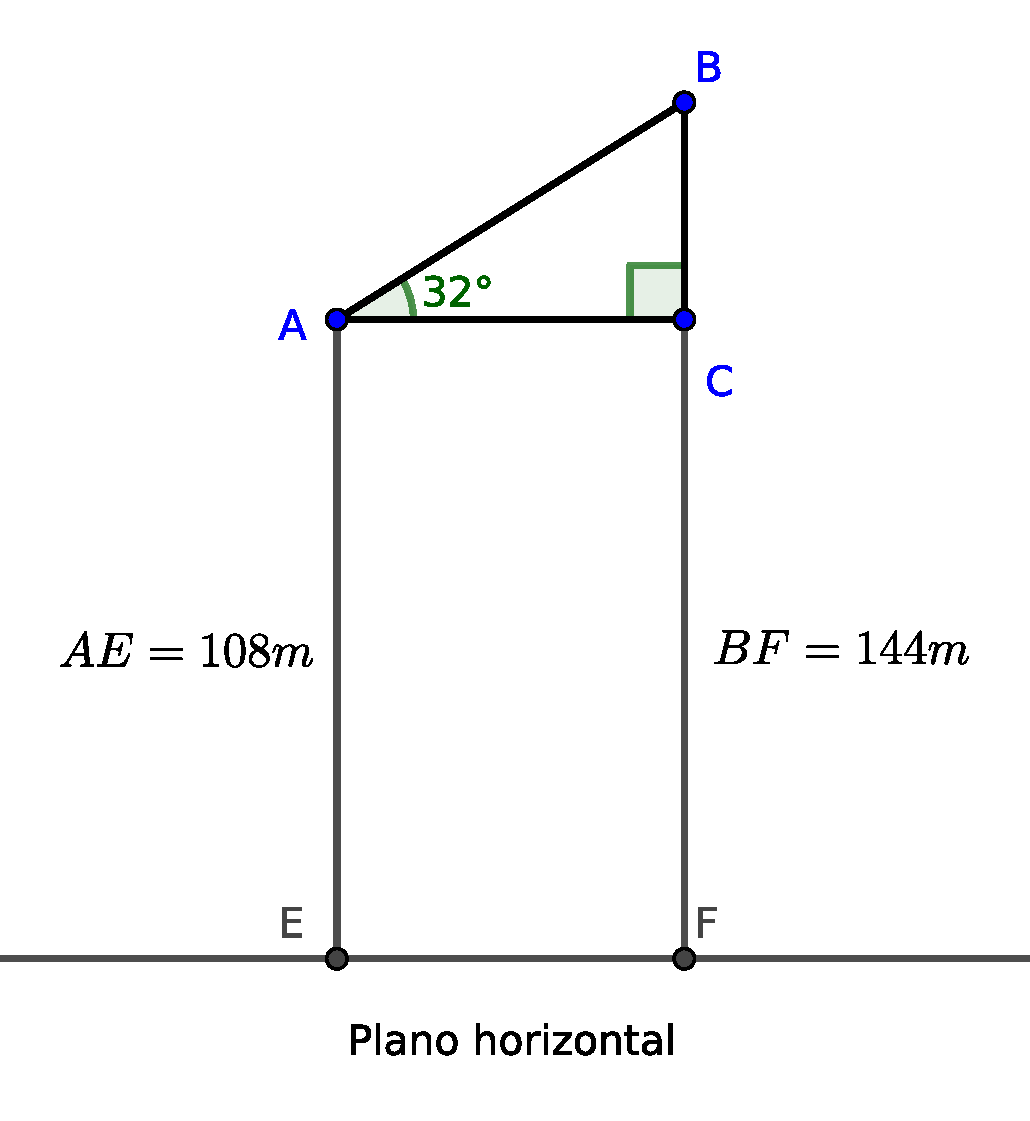
\includegraphics[width=5cm]{../../Topicos/Figuras/tri_ret_exer3.pdf}

 \end{multicols}


 \item (Sociesc - 2010) No retângulo abaixo retirou-se dos cantos quatro triângulos retângulos sombreados, formando assim um hexágono regular de lado 4cm.
  \begin{figure}[H]
   \centering
   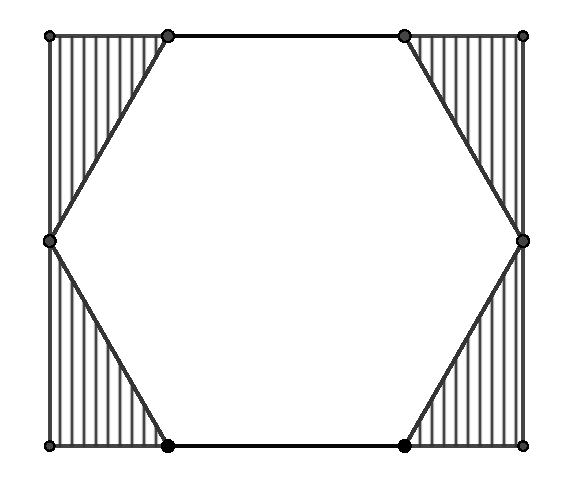
\includegraphics[width=5cm]{../../Topicos/Figuras/Hexagono.pdf}
  \end{figure}


  A área do retângulo é:
  \begin{enumerate}
  \item $64cm^2$
  \item $12\sqrt{3}cm^2$
  \item $48cm^2$
  \item $32\sqrt{3}cm^2$
 \end{enumerate}

 {\color{red} Nota:} cada ângulo interno de um hexágono mede $120\degree$.
 Pois,
 \vskip0.3cm
\colorbox{azul}{
 \begin{minipage}{0.9\linewidth}
 \begin{center}
 A soma dos ângulos internos de um polígono regular de $n$ lados é dada por:
  \[S= (n-2)\cdot 180 \degree .\]
 \end{center}
 \end{minipage}}
 \vskip0.3cm
 assim, como o hexágono é um polígono regular de $n= 6$ lados, decorre que a soma de seus ângulos internos é:
 \[S= (6-2)\cdot 180= 4 \cdot 180= 720 \degree\]
 portanto, cada ângulo interno $\alpha$ do hexágono mede:
 \[\alpha= \frac{720}{6}= 120 \degree .\]


 \end{enumerate}

 Gabarito: 1 d); 2 c); 3 c); 4 d).
